\documentclass{../main.tex}{subfiles}
\begin{document}
\chapter{TCP连接管理}
\section{引言}
TCP是一种\emph{面向连接}的单播协议。
在发送数据之前,通信双方必须在彼此间建立一条连接。
本章将详细地介绍TCP连接的概念,以及它的建立与终止过程。
如前文所述,TCP服务模型是一个字节流。
TCP必须检测并修补所有在IP层(或下面的层)产生的数据传输问题,比如丢包、重复以及错误。

由于需要对连接状态进行管理(通信双方都需要维护连接的信息),TCP被认为是一个比UDP(第10章)复杂的多的协议。
UDP是一种无连接的协议,因此它不需要连接的建立和终止过程。
与UDP相比,TCP在妥善处理多种TCP状态时需要面对大量的细节问题,
    比如一个连接何时建立、正常地终止、以及在无警告的情况下重新启动。
因此,这也被认为是两个协议的主要区别之一。
在后续章节,我们将探讨一旦建立连接并传输数据将会发生什么。

在连接的过程中中。通信双方需要交换一些选项。
这些选项被认为是连接的参数。
一些选项只被允许在连接建立时发送,而其他一些选项则能够稍后发送。
根据第12章的介绍,TCP头部已设置了一个有限的空间(40字节)来处理这些选项。


\section{TCP连接的建立与终止}
一个TCP连接由一个4元组构成,它们分别是两个IP地址和两个端口号。
更准确地说,一个TCP连接是由一对端点或套接字构成,其中通信的每一端都由一对(IP地址、端口号)所唯一标识。

一个TCP连接通常分为3个阶段: 启动、数据传输(也称为``连接已建立'')和推出(关闭)。
下文我们将会发现正确地处理上述三个阶段之间的转换是创建一个强健的TCP连接的困难所在。
图\ref{fig:create-destroy-connection}显示了一个典型的TCP连接的建立和关闭过程(不包括任何数据传输)。

图\ref{fig:create-destroy-connection}中的时间轴描绘了一个连接建立改成的相关事宜。为了建立一个TCP连接,需要完成以下步骤:
\begin{enumerate}
    \item 主动开启者(通常称为客户端)发送一个SYN报文段(即一个在TCP头部的SYN位字段置位的TCP/IP数据包),
        并指明自己想要连接的端口号和它的客户端初始序列号(记为ISN(c),参见13.2.3节)。
        通常,客户端还会借此发送一个或多个选项(参见13.3节)。客户端需发送的这个SYN报文段称作段1。
    \item 服务器也发送自己的SYN报文段作为响应,并包含了它的初始序列号(记为ISN(s))。该段称作段2。
        此外,为了确认客户端的SYN,服务器将其包含的ISN(c)数值+1后作为返回的ACK数值。
        因此,每发送一个SYN,序列号就会自动加1。这样如果出现丢失的情况,该SYN段将会重传。
    \item 为了确认服务器的SYN,客户端将ISN(s)的数值+1后作为返回的ACK数值。这称作段3。    
\end{enumerate}
\begin{center}
    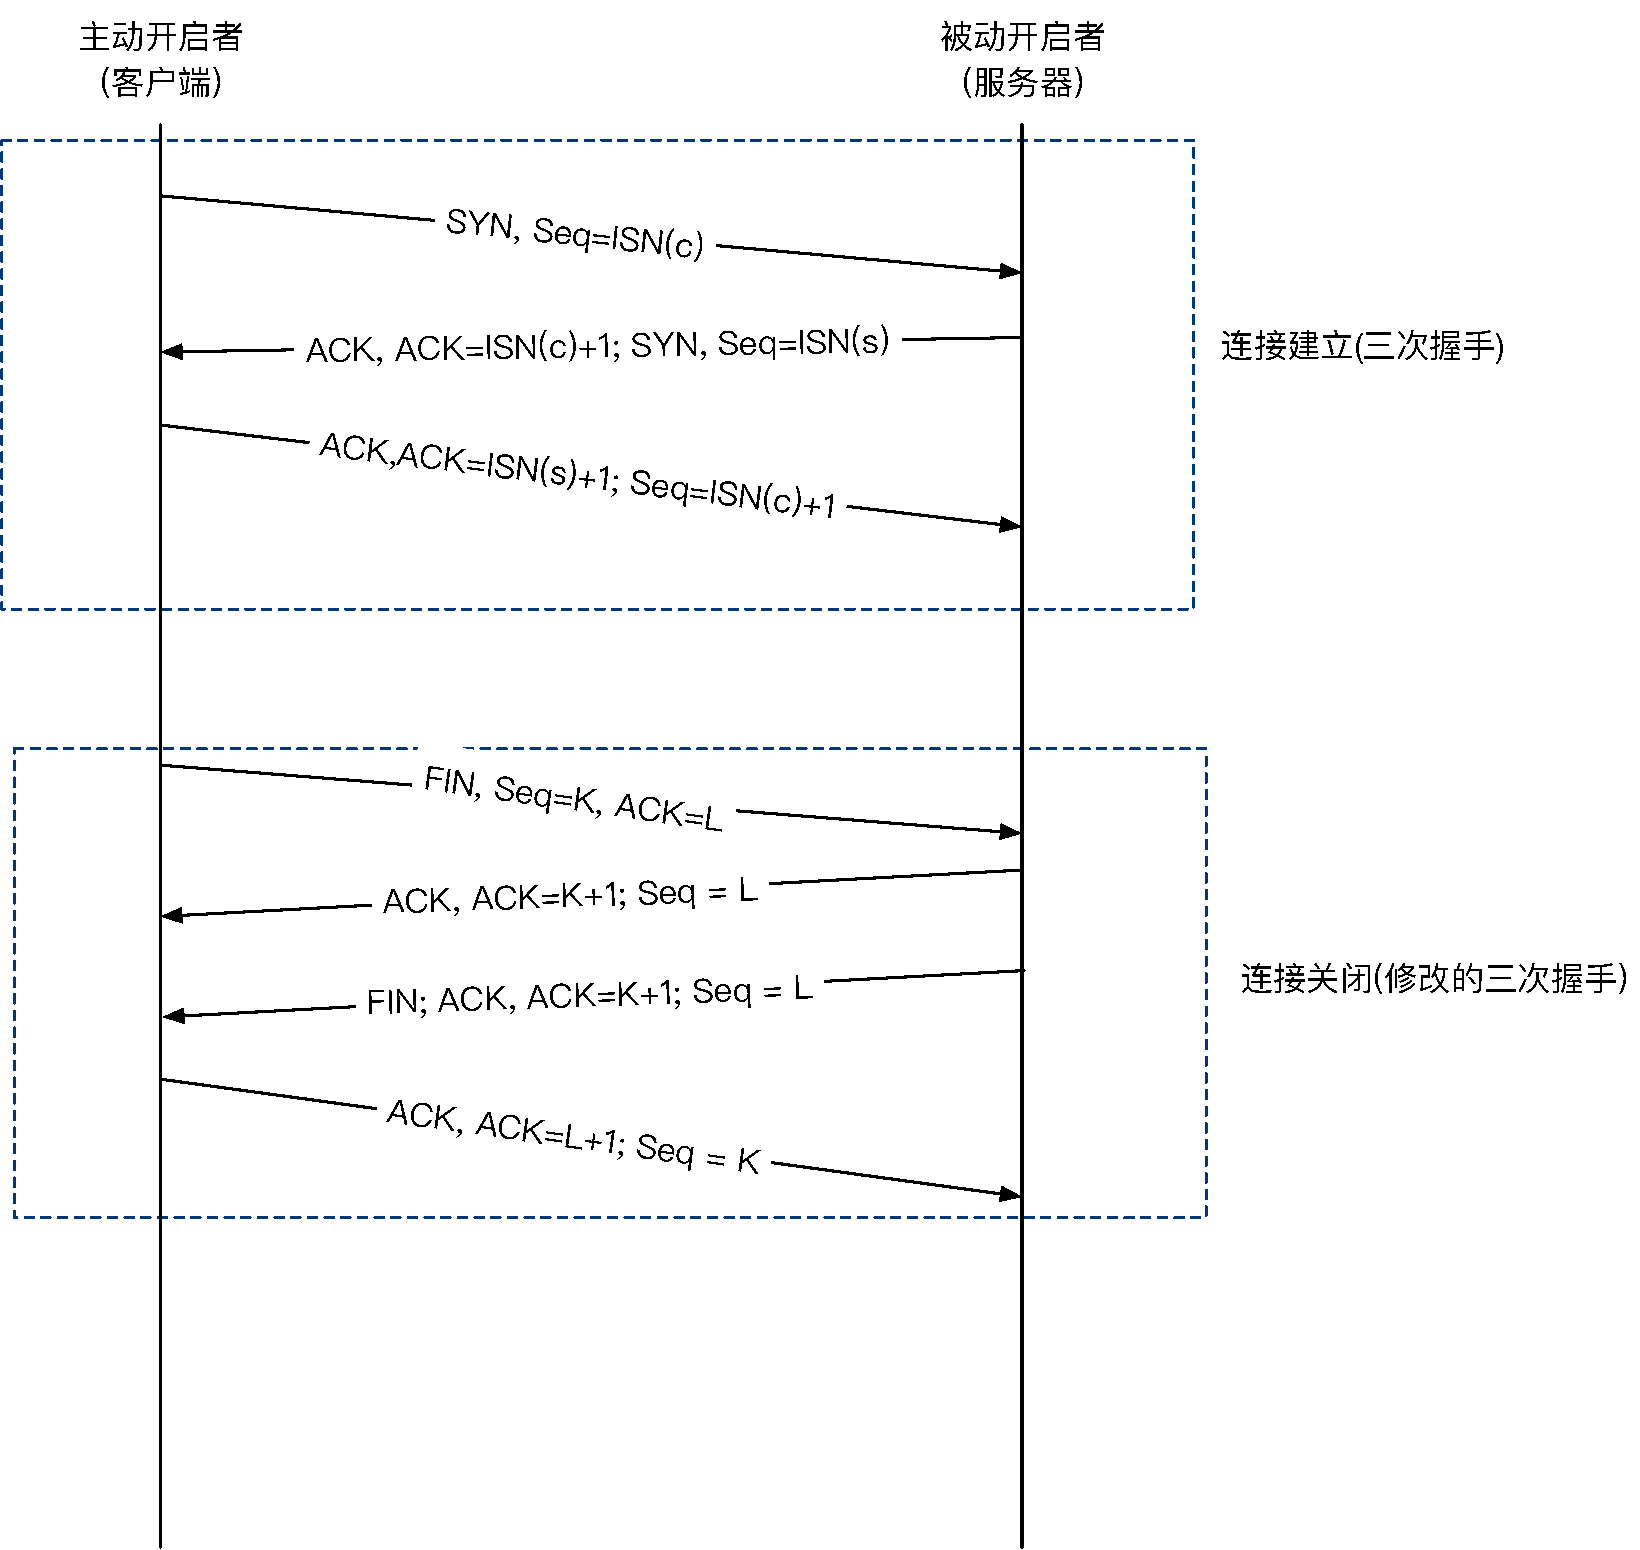
\includegraphics[width=0.8\textwidth]{resources/images/tcp-ip/create-destroy-connection.pdf}
    \captionof{figure}{
        一个普通TCP连接的建立与终止
    }
    \label{fig:create-destroy-connection}
\end{center}

如图\ref{fig:create-destroy-connection}所示,在一个普通的TCP连接建立与终止中。
通常由客户端负责发起一个三次握手过程。
在该过程中,客户端与服务器利用SYN报文段交换彼此的初始序列号(包括客户端的初始序列号和服务器的初始序列号)。
在通信双方都发送了一个FIN数据包并收到来自对方的相应的确认数据包后,该连接终止。

通过发送上述3个报文段就能够完成一个TCP连接的建立。
它们也常称作\emph{三次握手}。
三次握手的目的不仅在于让通信双方了解一个连接正在建立,还在于利用数据包的选项来承载特殊的信息,
    交换\emph{初始序列号(Initial Sequence Number, ISN)}。

发送首个SYN的一方被认为是主动地打开一个连接。
如上文所述,它通常是一个客户端。
连接的另一方会接收这个SYN,并发送下一个SYN,因此它是被动地打开一个连接。
通常,这一方称为服务器。
(13.2.2节将会介绍一种客户端与服务端同时打开一个连接的情况。这种情况可以作为上文所介绍内容的补充,但非常少见。)

\begin{tcolorbox}[title={注意}]
    TCP的SYN段也能够承载应用数据。
    由于伯克利套接字API不支持这种方式,因此它也很少为人所用。
\end{tcolorbox}

图\ref{fig:create-destroy-connection}还描绘了一个TCP连接是怎样关闭的(也称为清除或终止)。
连接的任何一方都能够发起一个关闭操作。
此外,该过程还支持双方同时关闭连接的操作,但这种情况非常少见。
在传统的情况下,负责发起关闭连接的通常是客户端(如图\ref{fig:create-destroy-connection}所示)。
然而,一些服务器(例如Web服务器)在对请求作出响应之后也会发起一个关闭操作。
通常一个关闭操作是由应用程序提出关闭连接的请求而引发的(例如使用系统调用close())。
TCP协议规定通过发送一个FIN段(即FIN位字段置位的TCP报文段)来发起关闭操作。
只有当连接双方都完成关闭操作后,才构成一个完整关闭:

1. 连接的主动关闭者发送一个FIN段指明接收者希望看到的自己的当前序列号($K$, 如图\ref{fig:create-destroy-connection}所示)。
FIN段还包含了一个ACK用于确认对方最近一次发来的数据(图\ref{fig:create-destroy-connection}中标记为L)。

2. 连接的\emph{被动关闭者}将$K$的数值加一作为响应的ACK值,
    以表明它已经成功接收到主动关闭者发送的FIN。
此时,上层的应用程序会被告知连接另一端已经提出了关闭的请求。
通常,这将导致应用程序发起自己的关闭操作。
接着,被动关闭者将身份转换为主动关闭者,并发送自己的FIN。该报文段的序列号为$L$。

3. 为了完成连接的关闭,最后发送的报文段还包含一个ACK用于确认上一个FIN。
值得注意的是,如果出现FIN丢失的情况,那么发送方将重新传输直到接收到一个ACK确认为止。

综上所述,建立一个TCP连接需要3个报文段,而关闭一个TCP连接需要4个报文段。
TCP协议还支持连接处于半开启状态(参见13.6.3节),但这种情况并不常见。
存在上述半开启状态的原因在于TCP的通信模型是双向的。
这也意味着在两个方向中可能会出现只有一个方向正在进行数据传输的情况。
TCP\emph{半关闭}操作是指仅关闭数据流的一个传输方向,而两个半关闭操作合在一起就能够关闭整个连接。
因此TCP协议规定通信的任何一方在完成数据发送任务后就能够发送一个FIN。
当通信的另一方接收到这个FIN时,就会告知应用程序对方已经终止了对应方向的数据传输。
由此可见,当程序发布关闭操作请求后,通信双方往往通过发送FIN段来关闭双向的数据传输。

如上文所述,7个报文段时每一个TCP连接在正常建立与关闭时的基本开销(下文还会介绍一些突然关闭TCP连接的方式)。
因此当只需要交换少量的数据时,一些应用程序更愿意选择在发送与接收数据之前不需要建立连接的UDP协议。
然而,这些应用程序也会面对由此引入的错误修复、拥塞管理以及流量控制等诸多问题。


\subsubsection{TCP半关闭}
如前文所述,TCP支持半关闭操作。
虽然一些应用需要此项功能,但它并不常见。
为了实现这一特性,API必须为应用程序提供一种基本的表达方式。
例如,应用程序表明``我已经完成了数据的发送工作,并发送一个FIN给对方,
    但是我仍然希望接收来自对方的数据直到它发送一个FIN给我''。
伯克利套接字的API提供了半关闭操作。
应用程序只需要调用shutdown()函数来代替基本的close()函数,就能实现上述操作。
然而,绝大部分应用程序仍然会调用close()函数来同时关闭一条连接的两个传输方向。
图13-2展示了一个正在使用的半关闭示例。
图中左侧的客户端负责发起半关闭操作,然而在实际应用中,通信的任何一方都能完成这项工作。

首先发送的两个报文段与TCP正常关闭完全相同:
初始者发送的FIN,接着是接收者回应该FIN的ACK。
由于接收到半关闭的一方仍能发送数据,因此图13-2中的后续操作与图\ref{fig:create-destroy-connection}不同。
虽然图13-2在ACK之后只描述了一个数据段的过程,
    但实际应用时可以传输任意数量的数据段(第15章将会详细地讨论数据段的交换与确认细节)
当接收半关闭的一方完成数据发送后,它将会发送一个FIN来关闭本方的连接,同时向发起半关闭的应用程序发出一个文件尾指示。
当第2个FIN被确认之后,整个连接完全关闭。 


\subsubsection{同时打开与关闭}
虽然两个应用程序同时主动打开连接看似不太可能,但是在特定安排的情况下是有可能实现的。
通信双方在接收到来自对方的SYN之前必须先发送一个SYN;
两个SYN必须通过网络送达对方。
该场景还要求通信双方都拥有一个IP地址与端口号,并且将其告知对方。
上述情况十分少见(第7章介绍的防火墙``打洞''技术除外),一旦发生,可称其为\emph{同时打开}。

例如,主机A的一个应用程序通过本地的7777端口向主机B的8888端口发送一个主动打开请求,
    与此同时主机B的一个应用程序也通过本地8888端口向主机A的7777端口提出一个主动打开请求,
    此时就会发生一个同时打开的情况。
这种情况不同于主机A的一个客户端连接主机B的一个服务器,
    而同时又有主机B的一个客户端连接主机A的一个服务器的情况。
在这种情况下,服务器始终是连接的被动打开者而非主动打开者,而各自的客户端也会选择不同的端口号打开。
因此,它们可以被区分为两个不同的TCP连接。
图13-3显示了在一个同时打开过程中报文段的交换情况。

一个同时打开过程需要交换4个报文段,比普通的三次握手增加了一个。
由于通信双方都扮演了客户端和服务器的角色,因此不能将任何一方称作客户端与服务器。
同时关闭并没有太大区别。
如前文所述,通信一方(通常是客户端,但不一定总是)提出主动关闭请求,并发送首个FIN。
在同时关闭中,通信双方都会完成上述工作。
图13-4显示了在一个同时关闭中需要交换的报文段。

同时关闭需要交换与正常关闭相同数量的报文段。两者真正的区别在于报文段序列是交叉的还是顺序的。
下文将会介绍TCP实现中同时打开与同时关闭操作使用特殊状态这一不常见的方法。


\subsubsection{初始序列号}
当一个连接打开时,任何拥有何时的IP地址、端口号、符合逻辑的序列号(即在窗口中)
    以及正确校验和的报文段都会被对方接收。
然而,这也引入了另外一个问题。
在一个连接中,TCP报文段在经过网络路由器后可能会存在延迟抵达与排序混乱的情况。
为了解决这一问题,需要仔细选择初始序列号。本届将详细介绍这一过程。

在发送用于建立连接的SYN之前,通信双方会选择一个初始序列号。
初始序列号随着时间改变而改变,因此每一个连接都拥有不同的初始序列号。
RFC0793指出初始序列号可被视为一个32位的计数器。
该计数器每4微妙加1。
此举的目的在于为一个连接的报文段安排序列号,以防止出现与其他连接的序列号重叠的情况。
尤其是对于同一连接的两个不同的实例而言,心的序列号也不能出现重叠的情况。

由于一个TCP连接是被一对端点所唯一标识的,其中包括由2个IP地址与2个端口构成的4元组,
    因此即便是同一个连接也会出现不同的实例。
如果连接由于某个报文段的长时间延迟而被关闭,然后又以相同的4元组被重新打开,
    那么可以相信延迟的报文段有会被视为有效数据而重新进入新连接的数据流中。
上述情况十分会令人十分烦恼。
通过采取一些步骤来避免连接实例间的序列号重叠问题,能否将风险降到最低。
即便如此,
    一个对数据完整性有较高要求的应用程序
    也可以在应用层利用CRC或校验和保证所需数据在传输过程中没有出现任何错误。
在任何情况下这都是一种很好的方法,并已普遍用于大文件传输。

如前文所述,一个TCP报文段只有同时具备连接的4元组与当前活动窗口的序列号,
    才会在通信过程中被对方认为是正确的。
然而,这也从另一个侧面反映了TCP的脆弱性:
如果选择合适的序列号、IP地址以及端口号,
    那么任何人都能伪造一个TCP报文段,从而打断TCP的正常连接。
一种抵御上述行为的方法是使初始化序列号(或者临时窗口号)变得相对难以猜出,
    而另一种方法则是加密(参见第18章)。

% Linux: 时钟 + 随机偏移量(散列函数生成,散列函数5min改变一次)
现代系统通常采用半随机的方法选择初始序列号。
证书报告CA-2001-09讨论了这一方法的具体实现细节。
Linux系统采用一个相对复杂的过程来选择它的初始序列号。
它采用了基于时钟的方案,并且针对每一个连接为时钟设置随机的偏移量。
随机偏移量是在连接标识(即4元组)的基础上利用加密散列函数得到的。
散列函数的输入每隔5分钟就会改变一次。
在32位初始序列号中,最高的8位是一个保密的序列号,而剩余的各位则由散列函数生成。
上述方法所生成的序列号很难被猜出,但依然会随着时间而逐步增加。
据报告显示,Windows系统使用了一种基于RC4的类似方案。


\subsubsection{例子}
前文介绍了一个TCP连接的建立和退出过程,本节将从数据包(分组)的角度进一步介绍相关细节。
为此我们尝试对邻近的Web服务器进行TCP连接。
该主机的IPv4地址为10.0.0.2,而客户端采用了基于Windows的Telnet应用。

telnet命令是建立在TCP连接的基础上的。
在上述例子中,该TCP连接必须与服务器的IPv4地址10.0.0.2以及http或Web服务的端口号(80端口)相关联。
当Telent应用程序连接23以外的端口(Telnet协议的众所周知端口以外的端口),它将不能用于应用协议。
它仅仅将自己的字节输入拷贝至TCP连接中,反之亦然。
当一个Web服务器接收到进入的连接请求时,它首先需要等待对Web页面的请求。
在这种情况下,我们不能提供这样的请求,因此服务器不会产生任何数据。
这些均符合我们的期望,因为我们只对连接建立与终止过程中的数据包交换感兴趣。
图13-5展示了Wireshark软件对该命令所产生的报文段的输出结果。

如图13-5所示,客户端发送的SYN报文段所包含的初始序列号为685506836,广告窗口为65535。
该报文段还包含了若干其他选项。
13.3节将详细地讨论这些选项。
第二个报文段既包含了服务器的SYN还包含了对客户端请求的ACK确认。
它的序列号(服务器的初始序列号)为1479690171,ACK为685506837。
ACK号仅比客户端的初始序列号大1,说明服务器已经成功接收到了客户端的初始序列号。
该报文段同样也包含了一个广告窗口以表明服务器愿意接收64240个字节。
第三个数据包将最终完成了三次握手,它的ACK号为1479690172。
ACK号是不断累积的,并且总是表明ACK发送者希望接收到的下一个序列号(而不是它上一个接收到的序列号)。

在4.4秒暂停后,Telnet应用程序被要求关闭连接。
这使得客户端发送第4个报文段FIN。
FIN的序列号为685506837,并由第5个报文段确认(ACK号为685506838)。
稍后,服务器会发送自己的FIN,对应的序列号为1479690172。
该报文段对客户的FIN进行了再次确认。
值得注意的是,该报文段的PSH位被置位。
虽然这样并不会对连接的关闭过程产生实质影响,但通常用于说明服务器将不会在发送任何数据。
最后一个报文段用于对服务器的FIN进行确认,ACK号为1479690173。
\begin{tcolorbox}[title={注意}]
    RFC1025将拥有最多特性(例如标记与选项)的报文段称为``神风''(kamikaze)数据包。
    其他生动的术语还包括``丑恶报文''、``圣诞树数据包''、``灯测试报文段''。
\end{tcolorbox}
从图13-5中我们还会发现SYN报文段包含了一个或多个选项。
这些选项需要占用TCP头部额外的空间。
例如,第一个TCP的头部长度为44字节,比最小的长度长24字节。
TCP也提供了若干选项,下文将详细介绍当一个连接无法建立时如何使用这些选项。


\subsubsection{连接建立超时}
本节的若干实例会展示连接不能建立的情况。
一种显而易见的情况是服务器关闭。
为了模拟这种情况,我们将telnet命令发送给一个处于同一子网的不存在的主机。
在不修改ARP表的情况下,上述做法会使客户端收到一个``无法到达主机''的错误消息后退出。
由于没有接收到针对之前发送的ARP请求而返回的ARP相应(第9章),
    因此会产生`无法到达主机''的消息。
如果我们能事先在ARP表中为这个不存在的主机添加一条记录,那么系统就不需要发送ARP请求,
而会马上根据TCP/IP协议尝试与这个不存在的主机建立联系。相关的命令如下: 
\todo[inline]{ARP命令}
上述例子选择的Mac地址00:00:1a:1b:1c:1d不能与局域网中其他主机的Mac冲突。
除此之外并无特例。
超时发生在发送命令后的3.2分钟。
由于没有主机响应,例子中所有的报文段都是客户端产生的。
清单13-1显示了使用Wireshark软件在摘要模式下获得的输出结果。
\todo[inline]{清单13-1}
有趣的是这些输出结果显示了客户端TCP为了建立连接频繁地发送SYN报文段。
在首个报文段发送后仅3秒第二个报文段就被发送出去,
    第三个报文段则是这之后的6秒,
    而第四个报文段则是在第三个报文段发送12秒以后被发送出去,
    以此类推。
这一行为被称作\emph{指数回退}。
在讨论以太网CSMA/CD介质访问控制协议时(参见第3章)我们也曾见过这样的行为。
然而,这两种指数回退也略有不同。
此处的每一次回退数值都是前一次数值的两倍,而在以太网中\emph{最大}的回退数值是上一次两倍,
    实际的回退数值则需要随机选取。

一些系统可以配置发送初始SYN的次数,但通常选择一个相对较小的数值5.
在Linux系统中,系统配置的$net.ipv4.tcp_syn_retries$表示了在一次主动打开
    申请中尝试重新连接发送SYN报文段的最大次数。
相应地,$net.ipv4.tcp_synack_retries$表示响应对方的一个主动打开请求时尝试重新发送ACK+SYN报文段的最大次数。
此外,它能够在设定Linux专有的$TCP_SYNCNT$套接字选项的基础上用于个人连接。
正如前面所介绍的,默认的数值为重试5次。
两次重新传输之间的指数回退时间是TCP用塞管理响应的一部分。
当我们讨论Karn算法时再仔细研究。


\subsubsection{连接与转换器}
在第7章,我们已经讨论了一些协议(比如TCP和UDP)如何利用传统的NAT转换地址与端口号。
我们还讨论了IP数据包如何在IPv6与IPv4两个版本间进行转换。
当TCP使用NAT时,伪头部的校验和通常需要调整(使用校验和中立地址修改器的情况除外)。
其他的协议也使用伪头部校验和,因为计算包含了与传输层、网络层相关的信息。

当一个TCP连接首次被建立时,NAT能够根据报文段的SYN位探明这一事实。
同样,可以通过检查SYN+ACK报文段和ACK报文段所包含的序列号来判断一个连接是否已经安全建立。
上述方法还适用于连接的终止。
通过在NAT中实现一部分TCP状态机(参见RFC6146的3.5.2.1与3.5.2.2)能够跟踪连接,
    包括当前状态、各方向的序列号以及相关的ACK号。
这种状态跟踪是典型的NAT实现方法。
当NAT扮演编辑者的角色并且向传输协议的数据负载中写入内容时,
就会涉及一些更复杂的问题。
对于TCP而言,它将会包括在数据流中添加与删除数据,
并由此影响序列号(与报文段)的长度。
此举会影响到校验和,但也会影响数据的顺序。
如果利用NAT的状态与终端主机的状态不同步,连接就无法正确进行下去。
因此,上述做法会到来一定的脆弱性。


\section{TCP选项}

\end{document}